\documentclass[12pt]{article}

%Packages add more power to LaTeX documents
\usepackage{fullpage} %Otherwise there will be a lot of wasted space at the margins
\usepackage{enumerate} %For the multi-part problem in example #4
\usepackage{amsthm} %For proof environment
\usepackage{amsmath} %For math symbols (like the black square)
\usepackage{graphicx,float,wrapfig} %Including graphics like PDFs and some image formats.
\usepackage{amssymb}
\usepackage{enumitem}
\newcommand\tab[1][1cm]{\hspace*{#1}}

\author{John E. Buckley III}
\title{CSCI 430: Homework 5}


\begin{document}
\maketitle

\section{3.1-1}

We need to prove the following inequations: \newline
\begin{enumerate}
\item c1(f(n)+g(n)) $\geq$ 0
\item c1(f(n)+g(n)) $\leq$ max(f(n), g(n))
\item max(f(n), g(n)) $\leq$ c2(f(n)+g(n)) \newline
\end{enumerate}
The \textbf{first} inequation holds since f(n) and g(n) are asymptotically non-negative functions which was stated in the problem. \newline \newline
The \textbf{second} inequation holds because max(f(n),g(n)) $\geq$ f(n) and max(f(n),g(n)) $\geq$g(n). This gives us max(f(n),g(n)) $\geq$ $\frac{(f(n)+g(n))}{2}$ \newline \newline
The \textbf{third} inequation holds because max(f(n),g(n)) $\leq$ f(n)+g(n). c2 $\geq$ 1.

\section{3.1-2}
\textbf{Proof:} There exists $n_0$ $\epsilon$ $ \mathbb{N}$ and there exists c1,c2 $\epsilon$ $\mathbb{R}$ s.t. for all n $\geq$ $n_0$: c1$n^b$ $\leq$ $(n+a)^b$ $\leq$ c2$n^b$. 
n+a$>$n because a$>$0 and n+a $\leq$ 2n for all n $\geq$ a. The inequalities are preserved by raising both sides by the power of b: (n+a)$>n^b$ and $(n+a)^b \leq 2^bn^b$. \newline 
Thus, this equation holds when $n_0$=a, c1=1, c2=$2^b$

\section{3.1-3}
Big O notation is usually used to indicate an upper bound of a function but the way the problem is worded,"is at least" which implies $\geq$, it actually gives us no information about the upper bound. The best running time could be anything slower than O($n^2$).

\section{3.1-4}
The first statement is true because: \newline
$2^{n+1}=2 \times 2^n \leq c2^n$ where c $\geq 2$. \newline \newline  
The second statement is false because: \newline
$2^{2n} \leq c \times 2^n$ \newline 
ln2 $\times$ 2n $\leq$ lnc+ln2 $\times$ n \newline
2n $\leq$ lnc+n \newline
n $\leq$ lnc 

\section{3.1-6}
If T(n)=$\Theta$(g(n)) then: 0 $\leq$ c1g(n) $\leq$ T(n) $\leq$ c2g(n) for n $\geq$ $n_0$ \newline
Since T(n) $>$ 0 and T(n) $\leq$ c2g(n): T(n)=O(g(n)) which is the upper bound or worst case running time. \newline
Since T(n) $\geq$ c1g(n) and c1g(n) $\geq$ 0: T(n)=$\Omega$(g(n)), which is the lower bound or best case running time.

\section{3.1-7}
From our notes, if we were to think calculus: \newline
f(n) is o(g(n)): $$\lim_{x\to\infty} \frac{f(n)}{g(n)}=0$$ \newline
f(n) is $\omega$(g(n)): $$\lim_{x\to\infty} \frac{f(n)}{g(n)}=\infty$$ \newline
Both of these cannot be simultaneously true, thus no f(n) exists.

\section{3.2-1}
From our notes, f(n) and g(n) are monotonically increasing iff n $\geq$ m $\rightarrow$ f(n),g(n) $\geq$ f(m),g(m). \newline \newline
Therefore: f(n)+g(n) $\geq$ f(m)+g(m): f(n)+g(n) is monotonically increasing \newline
Therefore: f(g(n)) $\geq$ f(g(m)): f(g(n)) is monotonically increasing \newline
Therefore: f(n) $\times$ g(n) $\geq$ f(m) $\times$ g(m): f(n) $\times$ g(n) is monotonically increasing 

\section{3.2-2}
Using the identities from our notes and some arithmetic: \newline
$a^{log_{b^c}}$ = $a^{log_{a^{\frac{c}{log_{a^b}}}}}$ \newline
\tab = $(a^{log_{a^c}})^{\frac{1}{log_{a^b}}}$ \newline 
\tab = $c^{frac{1}{log_{a^b}}}$ \newline
\tab = $c^{log_{b^a}}$ 

\section{3.2-3}
Using Stirling's approximation: \newline \newline
lg(n!) $\approx$ lg($\sqrt{2\pi n}$)($\frac{n}{e})^n)$ \newline
\tab = lg($\sqrt{2\pi n}$) + lg($\frac{n}{e})^n$ \newline
\tab = lg$\sqrt{2\pi}$ + lg$\sqrt{n}$ + nlg($\frac{n}{e}$) \newline
\tab = lg$\sqrt{2\pi}$ + $\frac{1}{2}lgn$ + nlgn - nlge \newline
\tab = $\Theta(1)$ + $\Theta(lgn)$ + $\Theta(nlgn)$ - $\Theta(n)$ \newline
\tab = $\Theta(nlgn)$ \newline \newline
n! = n $\times$ (n - 1) $\times$ (n - 2) $\times$ .... $<$ n $\times$ n $\times$ n .... n number of times, for n $\geq$ 2. \newline 
= o($n^n$) \newline \newline 
n! = n $\times$ (n - 1) $\times$ (n - 2) $\times$ .... $>$ 2 $\times$ 2 $\times$ 2 .... n number of times, for n $\geq$ 4. \newline
=$\omega(2^n)$ 

\section{3.2-6}
From our notes: we substitute $\phi$ and $\hat{\phi}^2$ and use some arithmetic.  \newline \newline
$\phi^2$ = ($\frac{1+\sqrt{5}}{2})^2$ \newline
= $\frac{1+2\sqrt{5}+5}{4}$ \newline
= $\frac{3+\sqrt{5}}{2}$ \newline
= $\frac{1+\sqrt{5}}{2}+1$ \newline
= $\phi$ + 1 \newline \newline
$\hat{\phi}^2$ = ($\frac{1-\sqrt{5}}{2})^2$ \newline
= $\frac{1-2\sqrt{5}+5}{4}$ \newline
= $\frac{3-\sqrt{5}}{2}$ \newline
= $\frac{1-\sqrt{5}}{2}+1$ \newline
= $\hat{\phi} + 1$

\section{3-2}
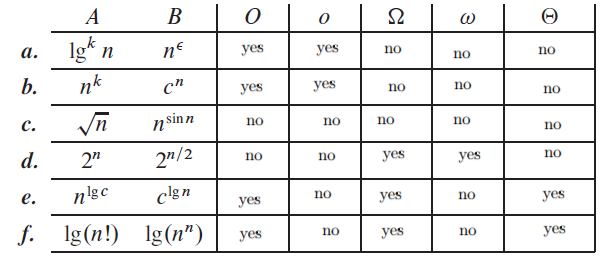
\includegraphics{3-2.png}

\begin{enumerate}[label=\alph*]

\item Polynomial grows faster than logarithm. \newline
\item Exponential grows faster than polynomial. \newline
\item No relations among them in terms of growth. \newline
\item Decreasing the base of an exponential function makes it grow slower. \newline
\item Both functions are same (see 3.2-2). \newline
\item Round the sum for $O$ and $\Omega$ and Stirling's Approximation for $\Theta$.

\end{enumerate}

\section{3-4}
\begin{enumerate}[label=\alph*]

\item False: Let f(n)=n and g(n)=$n^2$. n=$O(n^2)$ but $n^2 \neq O(n)$. \newline
\item False: Using the previous example: $n^2+n \neq \Theta(min(n^2,n))$. \newline
\item True: \newline
\item False: Let f(n)=2n and g(n)=n. f(n)=$O(g(n))$ but $n^{2n}=4^n \neq O(2^n)$. \newline
\item True: $ 0 \leq f(n) \leq cg(n) $ We need to prove that: $ 0 \leq df(n) \leq g(n) $ Which is straightforward with $d = 1/c$. \newline
\item False: Let f(n)=$4^n$. $4^n \neq \Theta(4(n/2))=\Theta(2^n)$. \newline
\item True: From our notes: $0 \leq o(f(n)) \leq f(n)$. Then $f(n) \leq f(n)+o(f(n)) \leq 2f(n)$. Thus, $f(n)+o(f(n))=\Theta(f(n))$.

\end{enumerate}

\end{document}